\clearpage
\section{Muons in jets \label{sec:muonjets}}
This section describes the special properties of jets containing muons. As mentioned in Section \ref{sec:samples}, a dedicated di-jet plus muon trigger has been used in data. The Monte Carlo samples are similar to the QCD samples used in the previous section except for the requirement of the presence of a muon at generator level.


Muons are
seeded from the CMS muon chambers, and are then linked to tracks found
in the tracking system to form global muons
\cite{JINST,CMS_PAS_MUO-10-002}.

The muon selection requirements are the following:
\begin{itemize}
\item transverse momentum $p_t >$ 7 GeV 
\item number of valid inner hits $>$ 10
\item number of pixel hits $>$ 1
\item number of missed outer hits $<$ 3
\item number of matches $>$ 0
\item inner $\chi^2 / ndof <$ 10
\item global  $\chi^2 / ndof <$ 10
\item longitudinal distance to primary vertex $<$ 2 cm
\item $\Delta$R to jet axis $<$ 0.4
\end{itemize}

Figure \ref{fig:muonplots1} shows the transverse momentum,  the impact parameter significance and the reconstructed number of muons per jet.


\begin{figure}[h!]
\centering
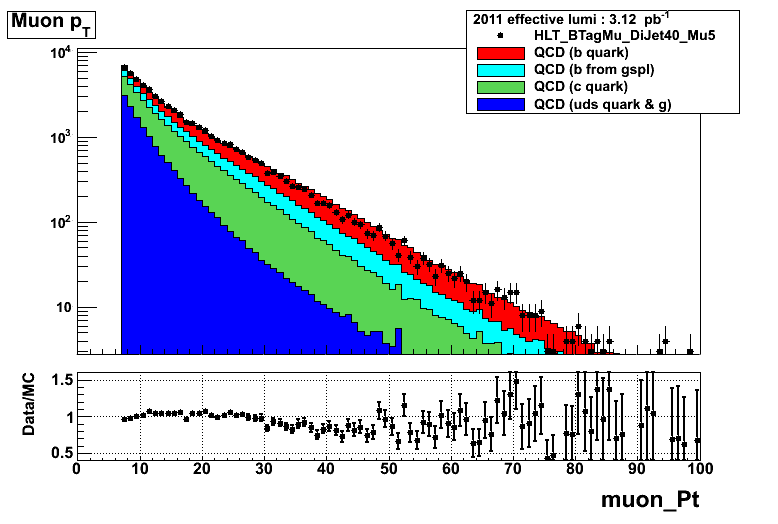
\includegraphics[width=0.32\textwidth]{figures/mujetmuon_Pt_Log.png}
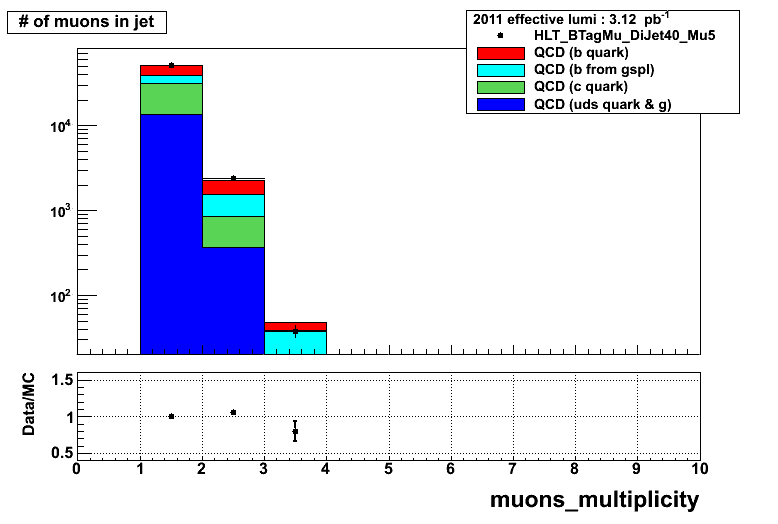
\includegraphics[width=0.32\textwidth]{figures/mujetmuons_multiplicity_Log.png}
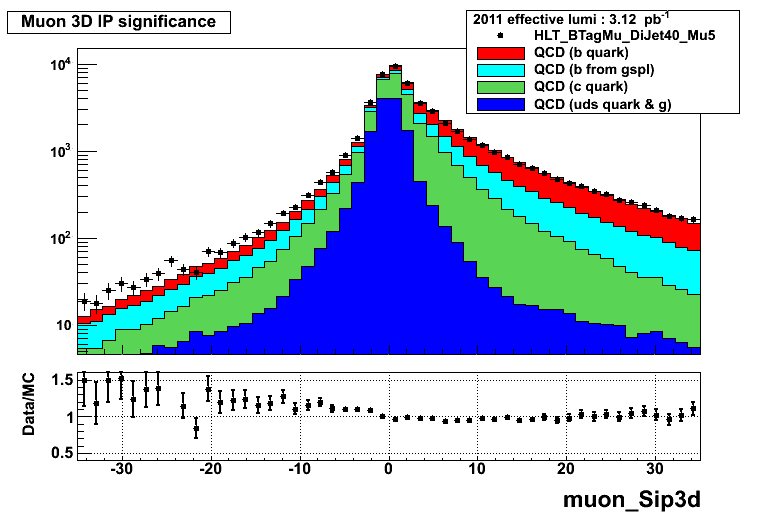
\includegraphics[width=0.32\textwidth]{figures/mujetmuon_Sip3d_Log.png}
\caption{Left: transverse momentum $p_t$ of muons in jets. Middle: number of reconstructed muons per jet. Right: 3D impact parameter significance of muons in jets.}
\label{fig:muonplots1}
\end{figure}



An important quantity for performance measurements is the relative transverse momentum with respect to the jet, $p_t^{rel}$. This is displayed in Figure \ref{fig:muonplots2} (left). There is an apparent discrepancy in this distribution which is also visible in the angle between the muon and the jet axis in units of $\Delta$R (Figure \ref{fig:muonplots2} right).

\begin{figure}[h!]
\centering
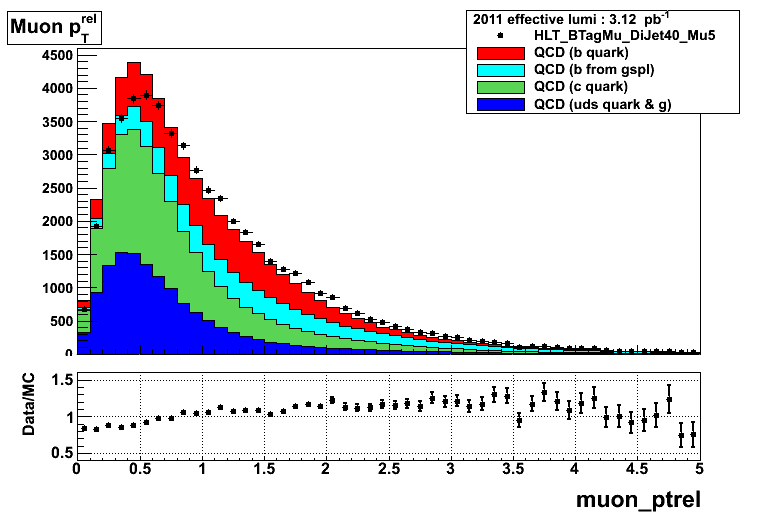
\includegraphics[width=0.42\textwidth]{figures/mujetmuon_ptrel_Linear.png}
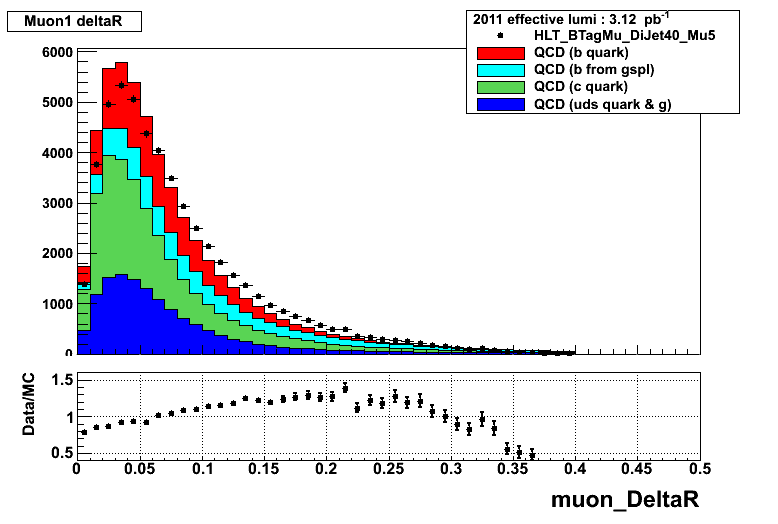
\includegraphics[width=0.42\textwidth]{figures/mujetmuon_DeltaR_Linear.png}
\caption{Left: transverse momentum of the muon with respect to the jet axis $p_t^{rel}$. Right: angle (in units of $\Delta R$) between the muon and the jet axis.}
\label{fig:muonplots2}
\end{figure}

The angular discrepancies in muon-jets are also visible in the secondary vertex angles. Figure \ref{fig:vertexAnglesMuJets}  shows the same distributions as Figure \ref{fig:vertexAngles}, but for jets with muons. The trend towards larger angles in data is enhanced in muon jets.

\begin{figure}[h!]
\centering
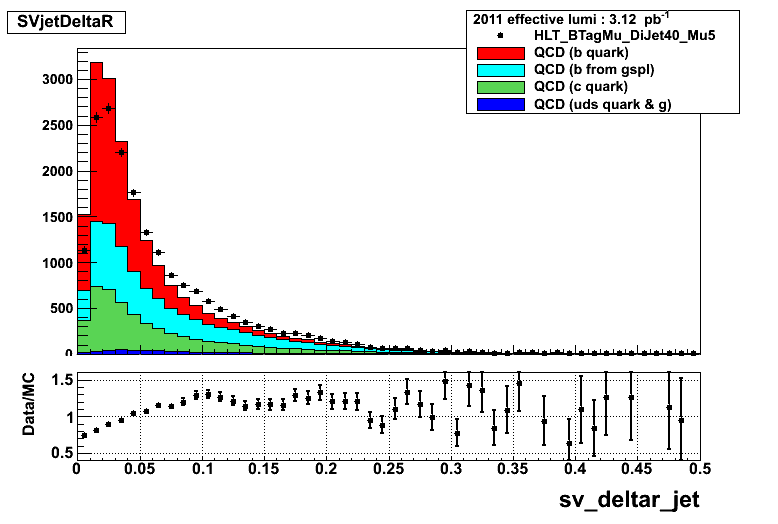
\includegraphics[width=0.32\textwidth]{figures/mujetsv_deltar_jet_Linear.png}
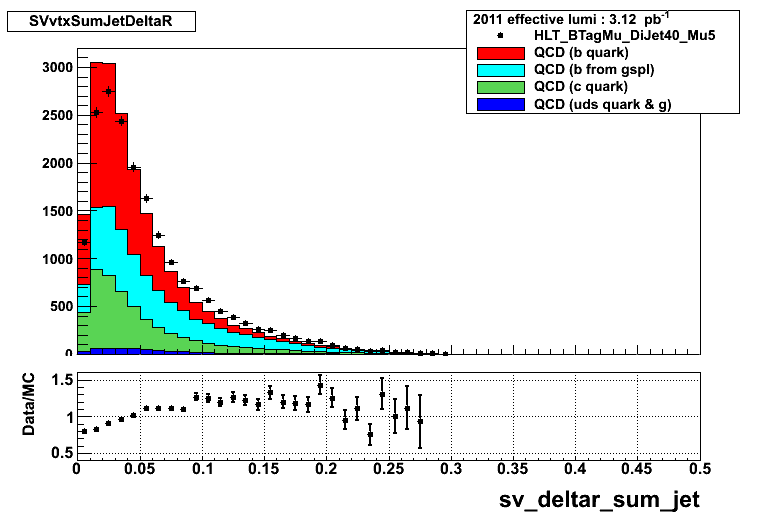
\includegraphics[width=0.32\textwidth]{figures/mujetsv_deltar_sum_jet_Linear.png}
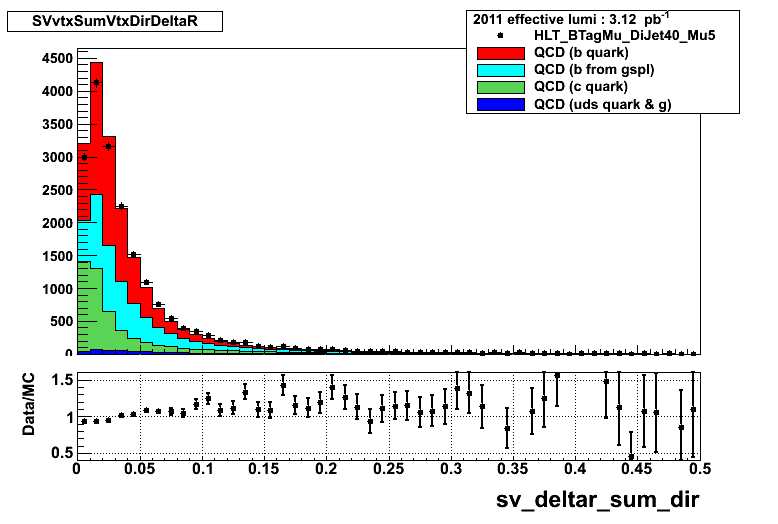
\includegraphics[width=0.32\textwidth]{figures/mujetsv_deltar_sum_dir_Linear.png}
\caption{Left: angular distance in $\Delta R$ between jet axis and vertex direction. Middle: angular distance in $\Delta R$ between jet axis and the sum of track momenta at the vertex, Right: angular distance in $\Delta R$ between vertex direction and the sum of track momenta at the vertex. }
\label{fig:vertexAnglesMuJets}
\end{figure}